\documentclass[12pt,a4paper,oneside]{article}
\usepackage[colorlinks=true,unicode]{hyperref}
\usepackage[utf8]{inputenc}
\usepackage[czech]{babel}
\usepackage{graphicx}
\usepackage{pdfpages}
\textwidth 16cm \textheight 25cm
\topmargin -1.3cm 
\oddsidemargin 0cm
\usepackage{footnote}
\pagestyle{empty}
\begin{document}
\title{Modul pro práci s procesory ARM řady STM32}
\author{Jakub Kákona, Miroslav Janás, kaklik@mlab.cz}
\maketitle

\thispagestyle{empty}
\begin{abstract}
\end{abstract}

\begin{figure} [htbp]
\begin{center}
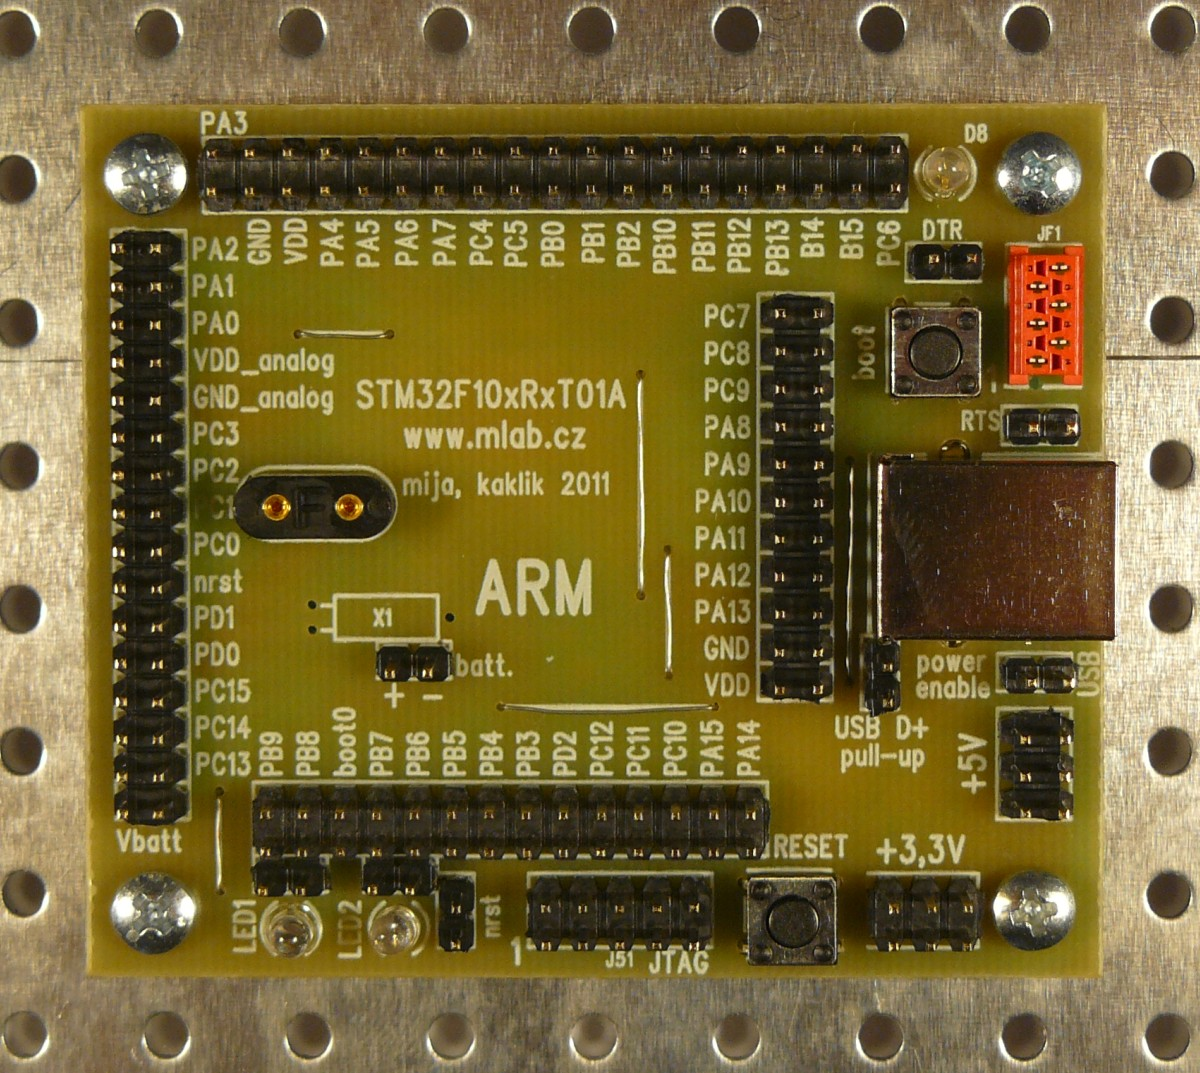
\includegraphics [width=80mm] {./img/STM32F10xRxT_Top_Big.jpg} 
\end{center}
\end{figure}

\begin{figure} [b]

\includegraphics [width=25mm] {./img/STM32F10xRxT_QRcode.png} 
\end{figure}

\newpage
\tableofcontents


\section{Technické parametry}
\begin{table}[htbp]
\begin{center}
\begin{tabular}{|c|c|c|}
\hline
\multicolumn{1}{|c|}{Parametr} & \multicolumn{1}{|c|}{Hodnota} & \multicolumn{1}{|c|}{Poznámka} \\ \hline
Napájecí napětí & +5V &  300mA \\ \hline
Progra  & $<$ 30dB & \\ \hline
\end{tabular}
\end{center}
\end{table}

\newpage
\section{Popis konstrukce}

\subsection{Zapojení}

Modul obsahuje CPU a základní součástky potřebné pro jeho funkci. Nahrávání firmware do modulu je možné přes několik rozhraní:

\begin{itemize}
  \item[USB] - nahrávání kódu přes USB se provádí utilitou dfu-util. Pro bližší informace viz wiki MLAB. 
  \item[UART] - stm32flash, Pro bližší informace viz wiki MLAB
  \item[JTAG] - OpenOCD, Pro bližší informace viz wiki MLAB.
\end{itemize}

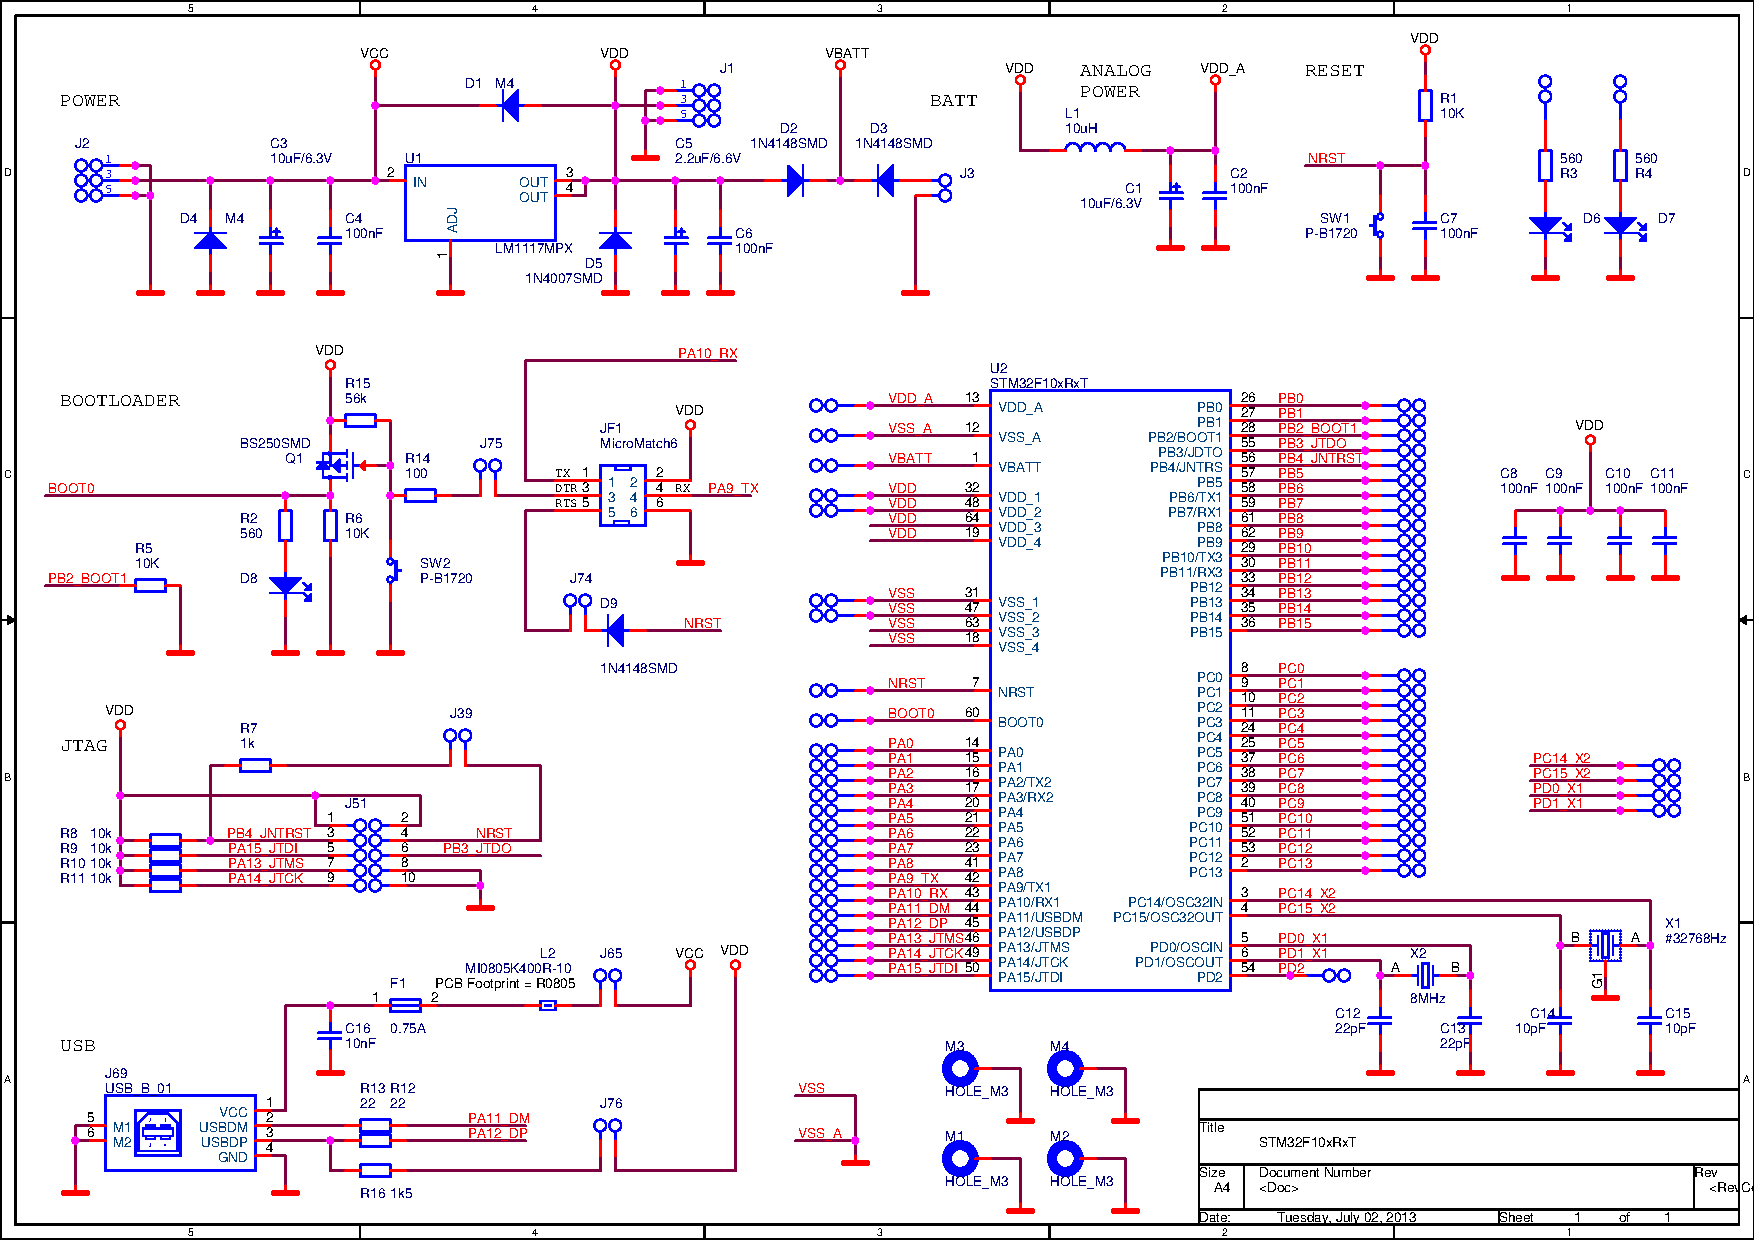
\includepdf[pages={1},landscape=true]{../../SCH/STM32F10xRxT.pdf}

\subsection{Odrušení}

Procesorový modul může být častou příčinou vzniku interferencí v elektronickém zařízení. Zvláště pokud zařízení obsahuje i analogové obvody pracujícími s malými signály. Je proto vhodné tento modul umisťovat odděleně od citlivých obvodů a tyto obvody z tohoto modulu nenapájet.

\section{Výroba a testování}

\subsection{Osazení}

\begin{figure} [h!tbp]
  \centering
  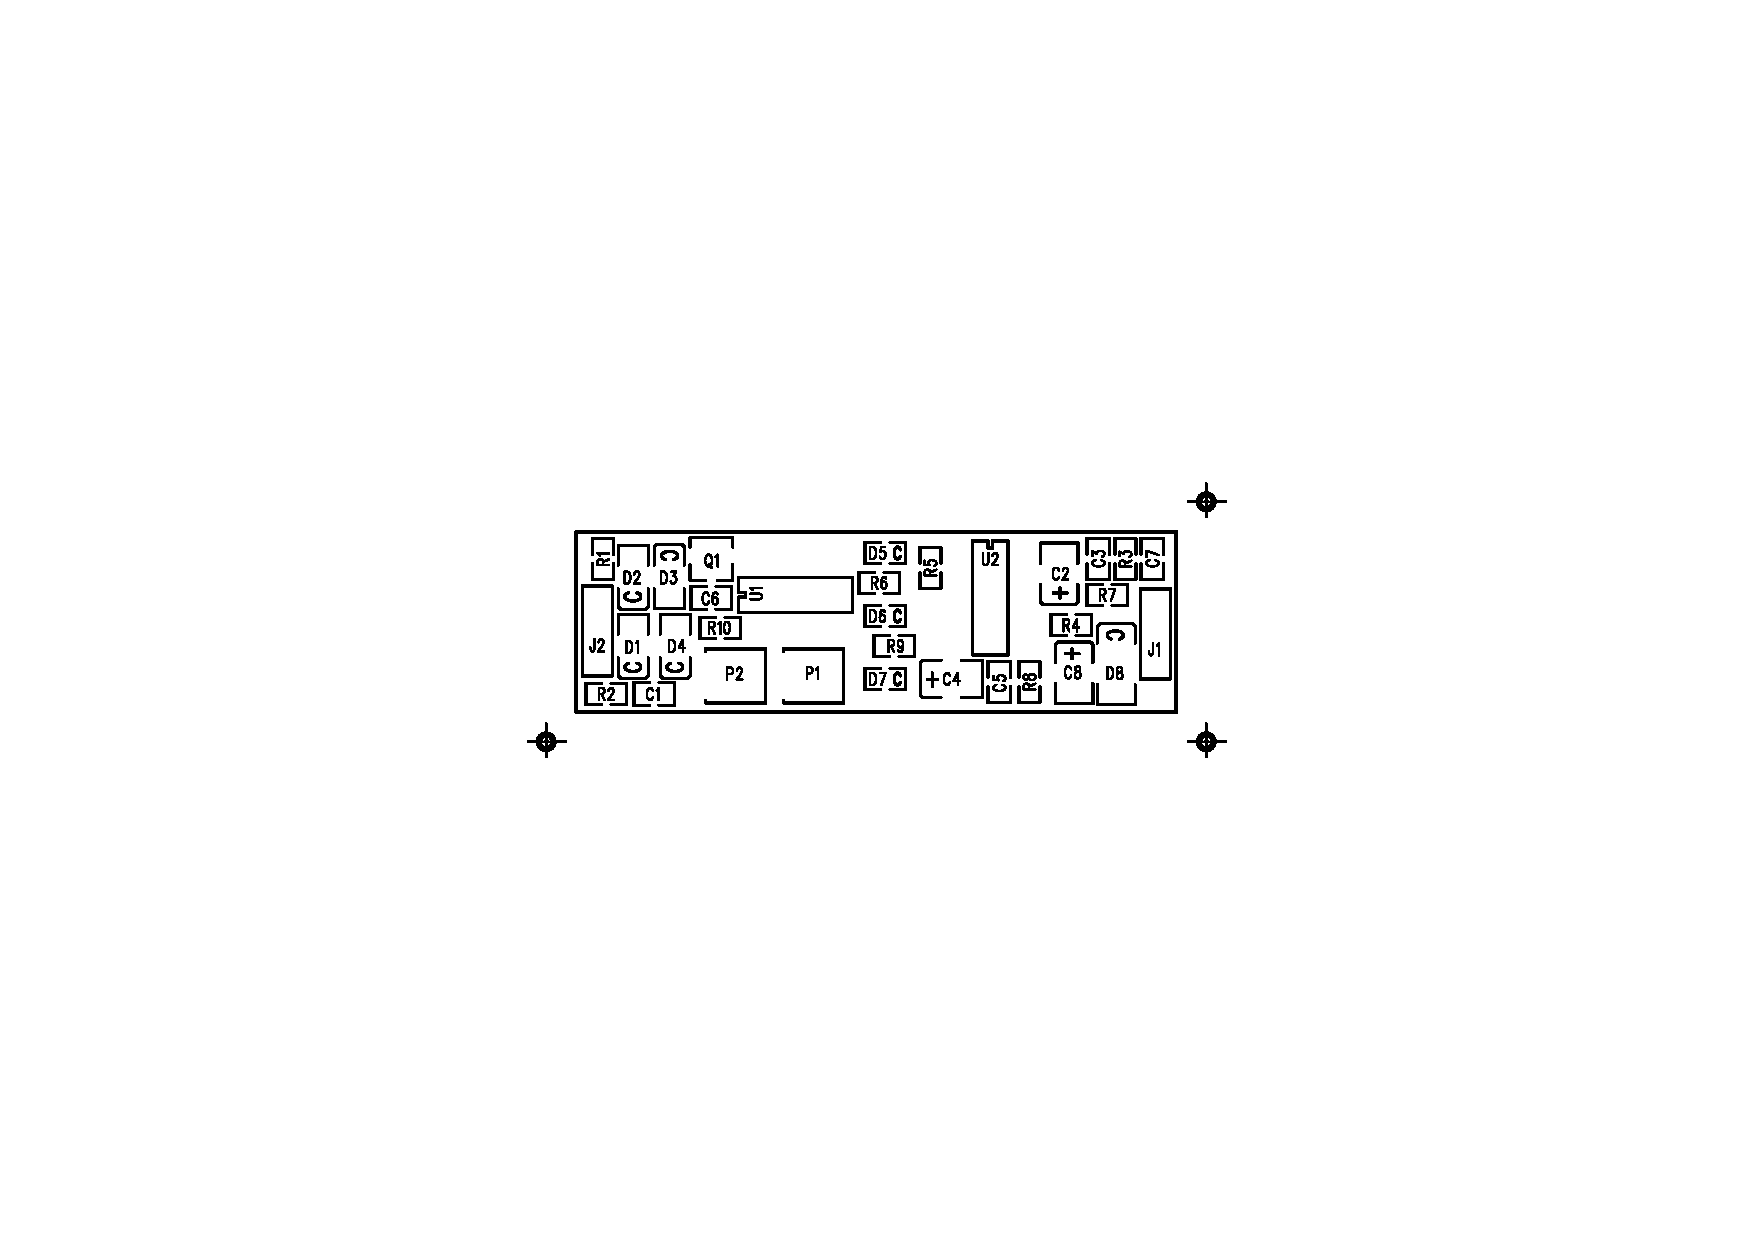
\includegraphics[trim = 6.5cm 11.5cm 6.5cm 11.5cm, clip, width=10cm]{../../CAM_DOC/O1.pdf}
  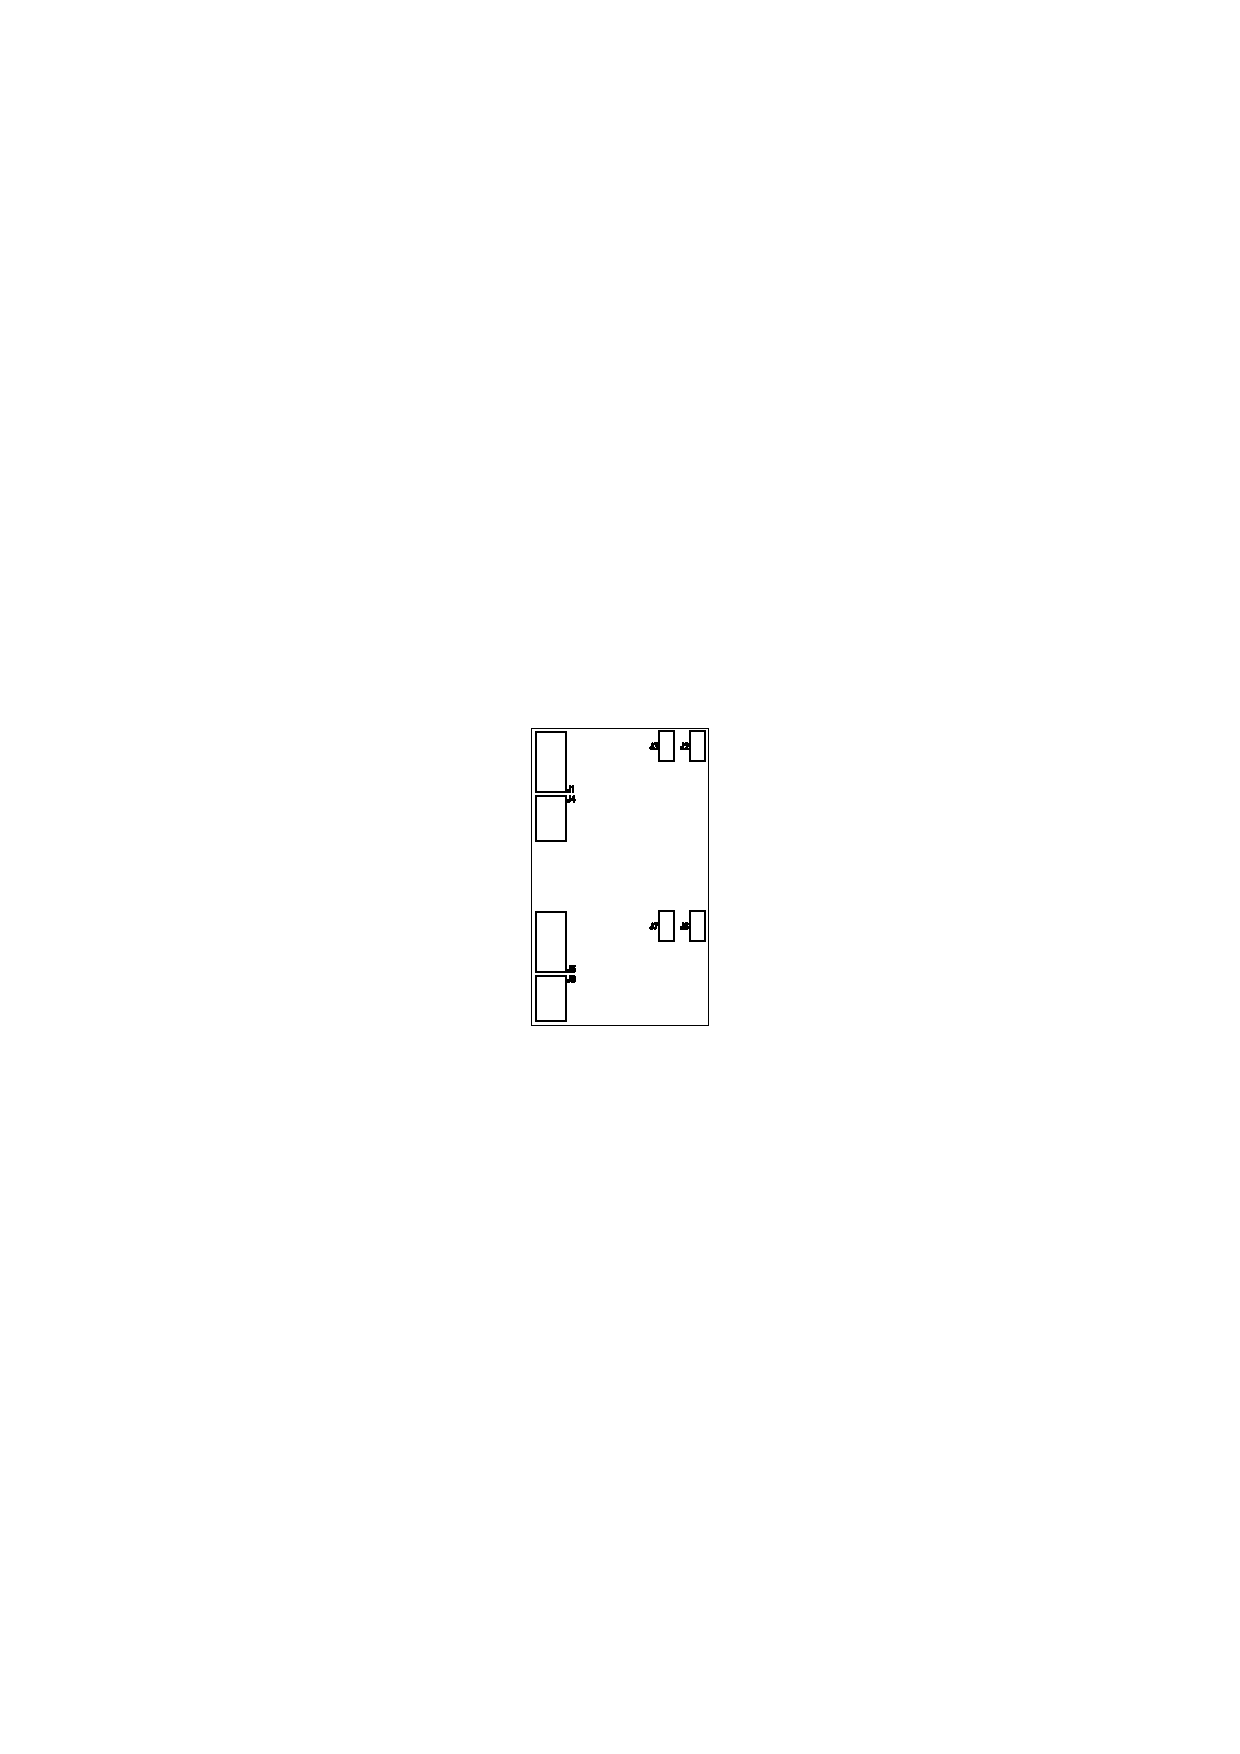
\includegraphics[trim = 6.5cm 11.5cm 6.5cm 11.5cm, clip, width=10cm]{../../CAM_DOC/O2.pdf}
  \caption{Osazovací plán horní a spodní strany plošného spoje}
  \label{fig:osazovaci_plan}
\end{figure}

\input{./STM32F10XRXT.BOM}

\section{Programové vybavení}


\begin{thebibliography}{99}
\bibitem{DR2G}{Původní konstrukce} 
\href{http:// odkaz na nejakou zajimavou konstrukci}{odkaz na nejakou zajimavou konstrukci}

\end{thebibliography}
\end{document}